\documentclass[../main.tex]{subfiles}


\begin{document}

In this chapter we will present our compression RNNs(C-RNN) designed to perform virtual sensing and provide reliable uncertainty estimates for its predictions. Recal we want to design virtual sensors  

Our general strategy is to use Recurrent Neural Networks(RNN) for modelling and prediction over time series data. 
The aleatoric uncertainty is modeled it as part of the phenomenon i.e. we learn to predict it from the data.
In terms of epistemic uncertainty, we focus on uncertainty stemming from OOD inputs, as we found in practice that it presents to biggest challenge for our applications. Our general strategy will be to model the training distribution $P(x)$, in order to be able to determine the likelihood of the input. That likelihood can then be used to estimate the epistemic uncertainty, or at least the component of it stemming from OOD inputs. Our models can be extended to account for parameter uncertainty by using techniques such as Monte-Carlo dropout\citep{gal2016dropout}. 

In the following subsections, we will begin by discussing how to model the training distribution, how to use that model to estimate epistemic uncertainty. Then we will present our full model, and how we train it.

\section{Modelling the training distribution}
\label{sec:information}

% Our approach to modelling the training distribution \pdf[train]{x} will be similar to variational autoencoders(VAE)~\citep{kingma2013auto}, adapted to sequential modelling. The only important difference is that the latent state for our model is deterministic. The main reason we use a deterministic latent state is speed. In typical deep learning 
Following the minimum description length principle\citep{rissanen1978modeling}, we model the data distribution by finding the model which compresses the data best. The link between data compression and distribution modelling is captured by the KL-divergence. Let \pdf{x|\theta} be a parameterized family of distributions, and \pdf[train]{x} be the distribution we wish to model. The KL-divergence
\begin{equation}
    \label{eq:kl}
    KL(\pdf[]{x} || \pdf{x|\theta}) = \int {\pdf[train]{x} log(\frac{\pdf[train]{x}}{\pdf{x|\theta}})} dx
\end{equation}{}
is equal to the expected number of additional bits required to compress the data from \pdf[train]{x} using \pdf{x|\theta}~\citep[chapter~5]{mackay2003information}. The KL hits its minimum of zero when the two distributions match exactly. Thus optimizing $\theta$ to minimize the number of bits required to compress the data is equivalent to minimizing the KL divergence between our family of distributions and the true distribution. 

Thus the task of modelling the distribution boils down to minimizing the expected number of bits required to compress data drawn from that distribution. We will use the training samples $X={x_1 \cdots x_n}$ to compute and optimize a monte-carlo estimate of that expectation. The KL becomes 
\begin{equation}
    \label{eq:mc_kl}
    KL(\pdf[]{x} || \pdf{x|\theta}) = - \frac{1}{N} \sum_{x \in X} log{(\pdf{x|\theta})} dx + const
\end{equation}{}

Thus we simply need to minimize the negative log likelihood of the training data, under our distribution. To define a flexible family of distributions we follow the approach taken in variational autoencoders~\citep{kingma2013auto}, which maps inputs from $X$ to a latent space $Z$ then maps latent codes $z$ back to the input space. A prior must be chosen over the latent state, typically a unit Gaussian~\citep{kingma2013auto}.

 The model consists of an encoder \pdf{z|x, \theta} and a decoder \pdf{x|z, \theta}. VAEs define \pdf{z|x, \theta} to be a Gaussian distribution, allowing the model to have a stochastic latent state. In the limiting case where the Gaussian is assumed to have infinitesimal variance, we can define \pdf{z|x, \theta} as a deterministic function~\cite{kingma2019introduction}. In this work we make this assumption, and treat the latent state as deterministic. Our motivation is having easier and faster training for our models. We found in initial experimentation that training recurrent models with stochastic latent states to be harder and more demanding computationally, while offering no tangible benefits.  

Let $\mathcal{H}$ denote the entropy~\citep{shannon1948mathematical} of a distribution and \pdf[prior]{z} a prior over the latent space, The loss function of a VAE\citep{kingma2013auto} is 
\begin{equation}
    \mathcal{L}_{VAE} = log(\pdf{x|z,\theta}) + log(\pdf[prior]{z}) - \mathcal{H}(\pdf{z|x, \theta})
\end{equation}{}

Assuming a deterministic latent state such that $\mathcal{H}(\pdf{z|x, \theta}) = 0$, the negative log-probability of an input $x$ under our model is
\begin{equation}
    \label{eq:logprob}
    -log(\pdf{x|\theta}) = -log(\pdf{x|z,\theta}) - log(\pdf[prior]{z})
\end{equation}{}

The first term $-log(\pdf{x|z,\theta})$ is our reconstruction cost after we map $x$ to some $z$ then reconstruct it. The second term $-log(\pdf[prior]{z|x,\theta})$ is the log-probability of the latent code $z$ the encoder assigns to $x$, under the prior \pdf[prior]{z}, we refer to it as the latent cost. 
Thus the loss we optimize in the end is 
\begin{equation}
        KL(\pdf[]{x} || \pdf{x|\theta}) = - \frac{1}{N} \sum_{x \in X} log(\pdf{x|z,\theta}) + log(\pdf[prior]{z})
\end{equation}{}
Thus the difference between our models and a VAE is that we use a deterministic state, and omit the entropy term from the loss. 

Once this model is trained, we use the negative log-probability of an input as the estimate of epistemic uncertainty
\begin{equation}
    \mathcal{E}(x) = -log(\pdf{x|\theta})
\end{equation}{}
Note that by Shannon's source coding theorem~\citep{shannon1948mathematical} the negative log probability of an outcome can be seen as the number of bits required to encode it~\citep{hinton1994autoencoders}. Thus $\mathcal{E}(x)$ is  the number of bits required to encode $x$ under the distribution defined by our model. 

The work we described so far did not involve any recurrence. In the recurrent case, we can exploit the temporal structure to define more flexible priors and achieve better compression. In general we can redefine \cref{eq:logprob} for temporal data 
\begin{equation}
    \label{eq:temporal_logprob}
    log(\pdf{x_t|\theta}) = log(\pdf{x_t|z_t,\theta}) + log(\pdf[prior]{z_t|z_{t-1}})
\end{equation}{}
We let the prior over $z$ at time $t$ depend on $z^{t-1}$, rather than having a static prior such as a unit Gaussian. In the next section we will detail our full approach, including how we defined flexible latent priors. 



% Suppose we are compressing points drawn from a distribution $Q(x)$, the ideal lossless compressor for this distribution, denoted here as $C_Q(x)$, takes any input $x$ and outputs a compressed $z$ where the length of $z$ is equal to the negative log probability of $x$
% \begin{equation}
%     \label{eq:compression}
%     len(z) = -log(Q(x))   
% \end{equation}{}
% Conversely, a probability model $Q(x)$ which assigns a probability $q$ to some point $x$, can be interpreted as assigning the input a compressed length of $-log(q)$. In short a probability distribution defines an ideal compressor and a compressor defines an ideal probability distribution. Note that this hold for lossless compression only, not lossy compression.  

% Let $C(x|\theta)$ represent a family of compressors parameterized by $\theta$. We have already established that a compressor can also be interpreted as a probability distribution over the input space, let $P(x|\theta)$ represent the distributions. The KL-divergence between $P(x|\theta)$ and the true data distribution $P(x)$
% \begin{equation}
%     KL(\pdf[]{x} || \pdf{x|\theta}) = \frac{1}{N} \sum_{x \in X}{P(x) log(\frac{P(x)}{P(x|\theta)})}
% \end{equation}{}
% is equal to the expected number of additional bits required to compress the data from $P(x)$ using $P(x|\theta)$~\citep[chapter~5]{mackay2003information}. The KL hits its minimum of zero when the two distributions match exactly. Thus optimizing $\theta$ to minimize the number of bits required to compress the data is equivalent to minimizing the KL divergence between our family of distributions and the true distribution. 

% % To have lossless compression, we need to account for the number of bits required to recover $x$ from the compressed code $z$ perfectly. 

% To learn compression models from data, we can train Autoencoders(AEs) which learn to compress inputs $x$ to compressed codes $z$ then reconstruct $x$. 
% The number of bits an AE needs to compress an input has two components, the number of bits in the compressed code, and the number of bits it takes to go from the model's reconstruction to the original input, since we require perfect reconstruction for this scheme to be sound.
% Those are commonly referred to as the likelihood and reconstruction loss respectively in the context of autoencoders. It is important to account for both, since it is trivial to compress data into short codes if we don't need to reconstruct it, and it is trivial to perfectly reconstruct data if we don't need to compress it.

% To optimize $\theta$ we do not need to actually generate the compressed codes and see how long they are, instead we can resort to probabilistic modeling again via \cref{eq:compression}. 
% For the compressed codes, we can define some prior probability distribution in some latent space, and let the model output a code in that space. The length of the code is then determined by the probability the prior assigns it again via \cref{eq:compression}, we call this $c_{l}(x)$. For the reconstruction error, instead of having the model output an exact reconstruction, we let the model output a probability distribution over the input space x, then the length of the code needed to specify the input exactly is also determined by the probability of the input under this distribution also via \cref{eq:compression}, we call this $c_{r}(x)$.

% To sum up the length of the compressed code word under for an input 
% \begin{equation}
%     \label{eq:compression_cost}
%     c(x) = c_{l}(x) + c_{r}(x)
% \end{equation}{}

% and the implied probability of the input is then $P(x|\theta) = 2^{-log(c(x))}$. 


\section{Compression RNNs(C-RNN)}
\label{sec:model}

\begin{figure}
    \centering
    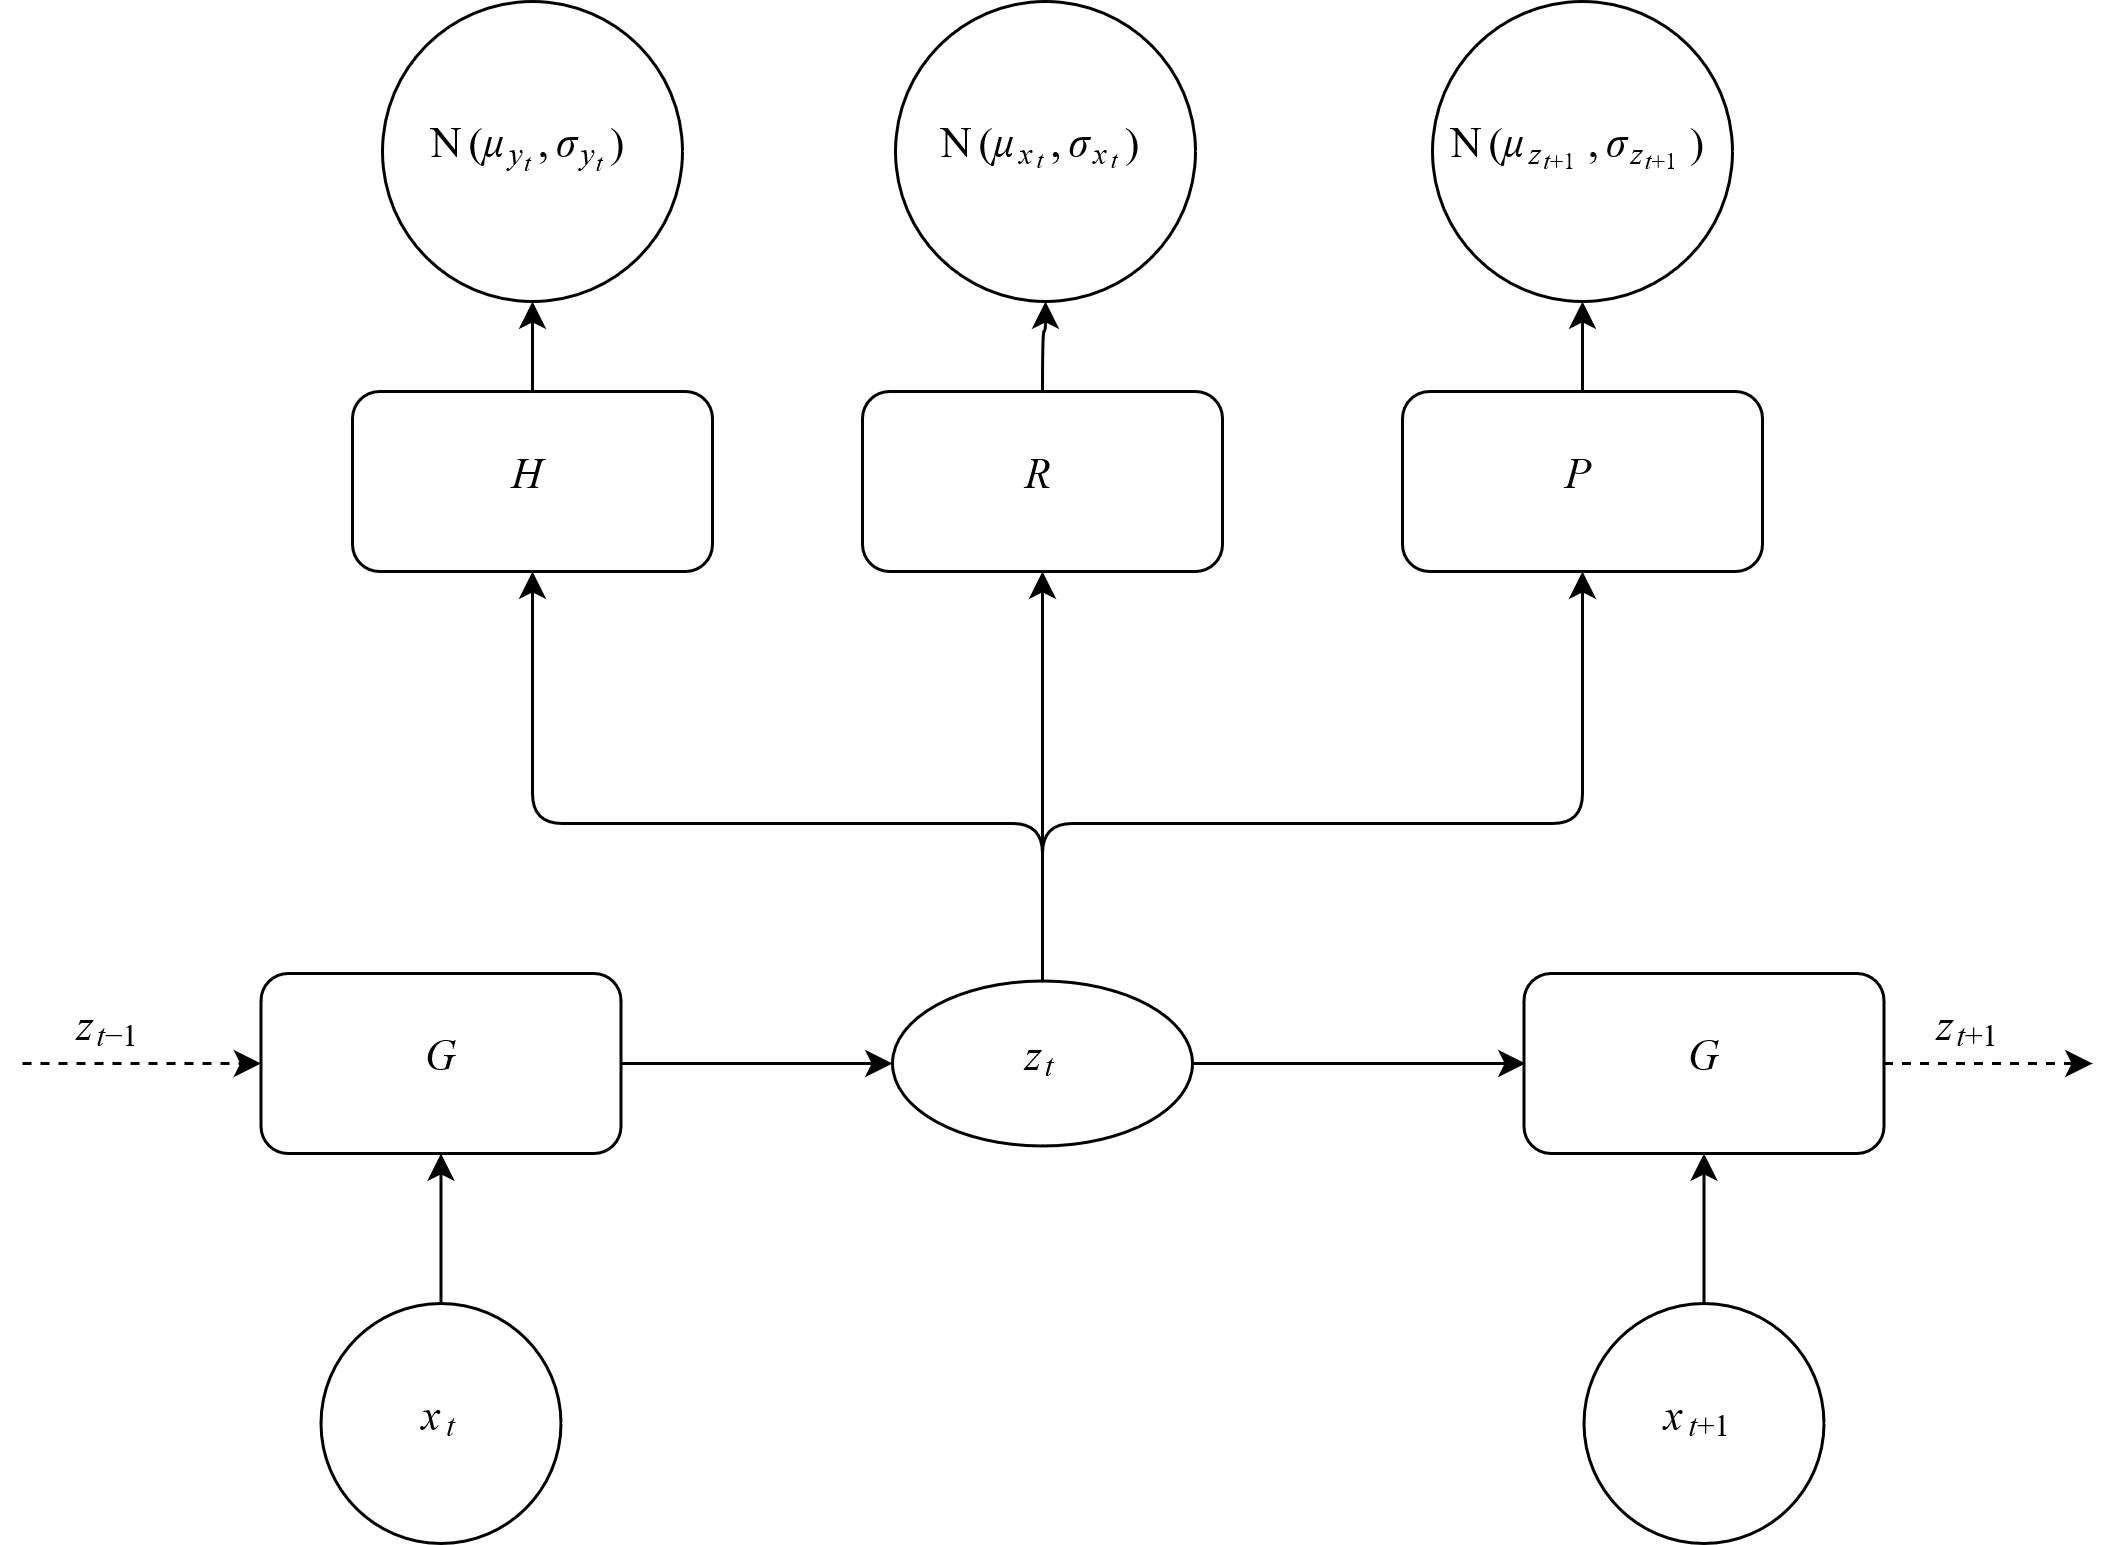
\includegraphics[width=\textwidth]{Approach/rnn_architecture.png}
    \caption{The C-RNN architecture, at each timestep the network outputs the mean and std of three Gaussians}
     \label{fig:architecture}
\end{figure}


\subsection{Model}

In this section we will introduce our compression RNN(C-RNN) which act as both the predictor for $y$ and density estimator for the training distribution \pdf[train]{x}. 
The architecture is depicted in \cref{fig:architecture}, The model is made up of four parameterized functions, all neural networks. Let $x_t$ denote our input at time t, $z_t$ our latent state, and $y_t$ our target and $\theta$ our model parameters.
\begin{enumerate}
    \item $g(x, z)$ is the recurrent module, which takes $z_{t-1}$ and $x_t$ to predict $z_t$
    \item $h(z)$ is the prediction module, which takes $z_t$ and predicts $y_t$
    \item $r(z)$ is the reconstruction module, which takes $z_t$ and predicts $x_t$
    \item $q(z)$ is the prior module, which takes $z_{t-1}$ and predicts $z_t$
\end{enumerate}

The prediction module outputs the model's predictive distribution for $y_t$ as a Gaussian distribution
$$
    h(z_t) = \pdf{y_t| x_t, \theta} = \mathcal{N}(\mu_{y_t}, \sigma_{y_t})
$$

The reconstruction module outputs the model's reconstruction of $x_t$
$$
    r(z_t) = \pdf{x_t| z_t, \theta} = \mathcal{N}(\mu_{x_t}, \sigma_{x_t})
$$

As discussed in the previous section(\ref{sec:information}), rather than define a static prior over the latent space, we define a flexible autoregressive prior to exploit the temporal structure of the data. Our prior for time $t$ is a Gaussian which depends on the previous latent state $z_{t-1}$. The prior module takes as input the previous latent state, then parameterizes a Gaussian which acts as a prior for time-step $t$
$$
    q(z_{t-1}) = \pdf[prior]{z_t} = \mathcal{N}(\mu_{z_t}, \sigma_{z_t})
$$
The prior is the model's prediction for the next latent $z_t$ state before $x_t$ is seen. 


\subsubsection{Uncertainty breakdown}
Our model estimates the aleatoric and epistemic uncertainty. The aleatoric uncertainty is encapsulated in $\sigma_{y_t}$ the variance of the model's predictive distribution.
We will use the shorthand $\mathcal{A}(x)$ to denote the model's aleatoric uncertainty
$$
    \mathcal{A}(x_t) = \sigma_{y_t}
$$

The epistemic uncertainty for an input is its compression cost or equivalently its negative log-probability under the model. We will use the shorthand $\mathcal{E}(x)$ to denote it, and it is computed by 
$$
    \mathcal{E}(x_t) = -log(\pdf{x_t|\theta}) = -[log(\mathcal{N}(x_t; \mu_{x_t}, \sigma_{x_t}) ) + log(\mathcal{N}(z_t; \mu_{z_t}, \sigma_{z_t})]
$$
This is a rewriting of \cref{eq:temporal_logprob} with our model's specific distributions. 

% \subsubsection{Implementation details}
% We use a GRU~\citep{cho2014learning} as we found them to preform best for our problems. We use leaky rectified linear units~\citep{nair2010rectified} for the hidden layer activations. 


\subsection{Training}
\subsubsection{Loss function}

Our loss function is composed of the prediction loss, and the compression loss. The prediction loss is the negative log-likelihood of the targets $y$
$$
    \mathcal{L}_y(x) =  -\log (\mathcal{N}(y; \; \mu_y, \sigma_y))
$$
The compression loss is composed of the reconstruction and latent costs
$$
    \mathcal{L}_c(x) = -[log(\mathcal{N}(x_t; \mu_{x_t}, \sigma_{x_t}) ) + log(\mathcal{N}(z_t; \mu_{z_t}, \sigma_{z_t})]
$$

Making our overall loss
\begin{equation}
    \label{eq:overall_loss}
    \mathcal{L}(x) = \mathcal{L}_{y}(x) + \lambda \mathcal{L}_c(x)
\end{equation}{}
Where $\lambda$ is a hyperparameter balancing the two components.

As our inputs are temporal sequences the loss decomposes such that for an $x={x_1 \cdots x_n}$ the overall loss
\begin{equation}
    \label{eq:detailed_loss}
    \mathcal{L}(x) = \sum_{t=1}^{n} -[\log (\mathcal{N}(y; \; \mu_y, \sigma_y)) + \lambda(log(\mathcal{N}(x_t; \mu_{x_t}, \sigma_{x_t}) ) + log(\mathcal{N}(z_t; \mu_{z_t}, \sigma_{z_t}))]
\end{equation}{}

The model is trained on mini-batches with the Adam optimizer~\citep{kingma2014adam}, following a cosine learning schedule~\citep{loshchilov2016sgdr}. However, we have made two modifications to improve the training.

\subsubsection{KL annealing}

A known issue for VAEs is KL-vanishing~\citep{bowman2015generating}, where early on in training the latent regularizer prevents the model from encoding information in the latent state, in order to push the latent loss down. We saw a similar problem in our setting, although our latent loss is an NLL loss. In our context it is also important to remember that we are not only autoencoding the inputs, but we are also making predictions. In fact the predictions are our main task. We found that when training the predictor and generative model as described, the predictive model is over-regularized and prediction quality goes down. Following~\citep{liu2019cyclical}, we use a cyclical annealing schedule for the compression loss. Specifically, our schedule is over $\lambda$ in \cref{eq:overall_loss}. The $\lambda$ parameter starts a cycle at zero and increases linearly, reaching its maximum at the mid point of the cycle, then remains constant for the rest of the cycle. Our experimental results show that KL annealing improves on both the prediction quality and the uncertainty estimation. 

\subsubsection{Compression loss weighting}

Our motivation for modelling the density of the training is distribution is to use it to determine how reliable our prediction is for an input, assuming our model performs well on points drawn from the training distribution.
If an input is likely under the training distribution, it would follow that our model is likely to give a good prediction for that input. The problem comes from that fact that our model may not be performing equally well over the whole training distribution. This may be due to bad priors, poor optimization, or simply the complexity of the behavior of $P(y|x)$ in certain regions. In short, the density of the training distribution may not be perfectly correlated with the model's performance. In order to get higher quality uncertainty estimates we wish to place more mass in the input regions where the model performs well, and less in regions where the model performs poorly. 

In order to bias our density estimator to place less mass in regions where the model performs poorly, we use a weighted compression loss, where points with high prediction loss get less weight. Recall our compression loss ${L}_c(x)$ minimizing the compression cost of the training inputs, which is equivalent to minimizing the negative log-likelihood of the training inputs, giving all the inputs equal weight. Far a mini-batch the loss is
\begin{equation}{}
    \mathcal{L}_c = \frac{1}{nm} \sum_{i=1}^n \sum_{t=1}^m \mathcal{L}_c(x^i_t) 
\end{equation}
for a batch with $n$ sequences of length $m$. We wish to add weights $w$ which give more importance the points where the model preforms well, and less importance to points where the model preforms poorly, such that the loss becomes

\begin{equation}
    \mathcal{L}_c  =  \sum_{i=1}^{n}  \sum_{t=1}^{m} w^i_t \; \mathcal{L}_c(x^i_t) 
\end{equation}
for a 

Where the $w^i_t$ are weights assigned according to how well the predictive model performs on that point i.e. how good the model's prediction for $y$ was. The weight $w^i_t$ should be large when the model predicts $y^i_t$  well from $x^i_t$ and low otherwise. The intuition here is consistent with \cite{theis2015note}, where the authors argued that the quality of a generative model is difficult to measure in an objective sense, and that rather the utility of generative models depends on how well they preform on the downstream tasks they are intended for. We take this intuition not just for evaluation, but also for training our model. 


% The weights should depend on our predictive errors $\mathrm{E}$. Let $\mathrm{E} = |Y - \hat{Y}|$ be a vector containing absolute error of between our model predictions and the targets for a training mini-batch. Let $W$ be the vector containing our weight, we can define $W$ with 
% \begin{equation}
%     W = Softmax(\mathrm{E} \cdot t)
% \end{equation}{}

% Where t is a temperature hyperparameter. If we set $t$ to zero, we can get back the original formulation, and as we increase the temperature we can bias the model towards placing more mass in regions where the error is small.

We want to choose weights $w$ which encourage the behavior we want, and which is usable for training.  

\textbf{Decoupling uncertainties} We choose an unsigned Z-score as the error metric we derive the weights from. We define it as 
\begin{equation}
    Zs(x_t^i) = \frac{|y_t^i - \mu_{y_t^i}|}{\sigma_{y_t^i}}
\end{equation}{}
where $y_t^i$ is the ground truth target for sequence $i$ at time $t$, $\mu_{y_t^i}$ the model's prediction, and $\sigma_{y_t^i}$ the model's aleatoric uncertainty. Our motivation for choosing this metric is that it captures the relationship between model errors and aleatoric uncertainty. We want the epistemic uncertainty to be highest when the error is large and the aleatoric uncertainty is small, and this is when the Z-score is highest. If both the error and aleatoric uncertainty are high, we can consider the error covered by the aleatoric uncertainty. This decouples the aleatoric and epistemic uncertainty to an extent.

We need to compute weights from the Z-score such that points with higher Z-score get lower weights. One solution could be to use the inverse, however that could be unstable. Instead we resort to a softmax over the negative Z-score. 
$$
    w_i^t = softmax(-Zs(x_t^i))
$$
The softmax guarantees positives weights which sum to one. This makes it an appealing choice for optimization so that the norm of the gradient does not change violently because of the weights, since the overall weight assigned to the batch is always one. 



\end{document}
